\section{Hauptteil}
\label{sec:hauptteil}

\subsection{Auswirkungen des Semantischen Webs auf die Wirtschaft}

\subsection{Auswirkungen des Semantischen Webs auf die Gesellschaft}

Schon heute drehen sich die meisten der regelmäßig ausgeführtem Aktivitäten im Internet um \buzz{Informationen} oder gar \buzz{Wissen}, nicht um \buzz{Daten}. So sind 56\% der im Digitalindex 2014 befragten Deutschen überzeugt, im Internet die automatisch die aktuellsten Informationen zu finden, 60\% sucht benötigte Informationen zuerst im Netz\footnote{vgl. \cite{d21}, Seite 6}. Die Erwartungen bzgl. Aktualität und Informationsgehalt an das \ac{WWW} sind also sehr hoch. 

\begin{figure}[H]
\begin{center}
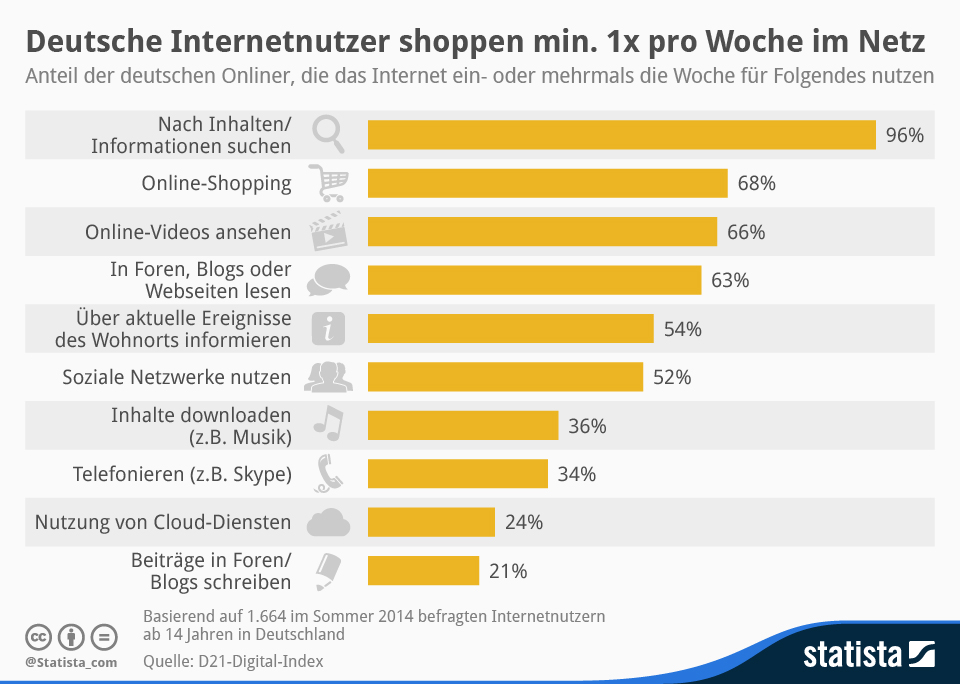
\includegraphics[width=0.67\textwidth]{inetnutzung.jpg}
\caption[Internetnutzung in Deutschland 2014]{Internetnutzung in Deutschland 2014\protect\footnotemark}
\label{pic:inetnutzung}
\end{center}
\end{figure}
\footnotetext{\cite{d21}, Seite 37}


Unter den Top 10 der regelmäßig durchgeführten Tätigkeiten der Befragten im Web finden sich die informationsorientierten Tätigkeiten „nach Inhalten/Informationen suchen“ auf Platz eins, „über aktuelle Ereignisse des Wohnorts informieren“ auf Platz 6 und die Erfassung eigener Daten auf Platz 10\footnote{vgl. \cite{d21}, Seite 37}. Weitere Tätigkeiten wie „Soziale Netzwerke nutzen“ (Platz 7) bzw. „Online--Videos ansehen“ (Platz 3) sowie „Online--Shopping“ (Platz 2) nutzen Internetangebote, die per Design sehr gut mit Taxonomien, Meta--Daten und Verknüpfungen ausgestattet sind.

Neben dem offensichtlichen Nutzen des \ac{WWW} bringt die Entwicklung des Webs auch negative Auswirkungen auf die Gesellschaft. 
Dies äußert sich mit der Besorgnis von 60\% der Nutzer über die im Internet möglicherweise verfügbaren persönlichen Daten\footnote{vgl. \cite{d21}, Seite 6}. 

Man kann davon ausgehen, dass mit weiter wachsenden Datenmengen, aber auch durch entsprechenden Wachstum an generierten und erfassten Informationen und Wissen sowohl die positiven Erwartungen als auch die Befürchtungen und Ängste in der Bevölkerung zunehmen werden.


\subsection{Vergleich der Auswirkungen mit denen des Öls}

\subsection{}
